\documentclass{beamer}
\usepackage{beamerthemesplit}
\usepackage{booktabs}
\usepackage{graphicx}
\usepackage{transparent}
\usepackage{bbold}
\usepackage[italian]{babel}
\usepackage[utf8x]{inputenc}
\usepackage{listings}
\usepackage{tikz}
\usetikzlibrary{arrows}
\usepackage{amsmath,amsfonts,amssymb}
\usepackage{pgfplots}
\usepackage{scalefnt}
\usepackage{color}
\usepackage{xcolor}
\title[PAGERANK]{PageRank}
\institute{
\begin{small}
Corso di Laurea in Informatica Magistrale
\end{small}}
\author{\textbf{Simone Rutigliano}}
\date{\tiny{\today}}

\usebackgroundtemplate{
%    \transparent{0.12}{
     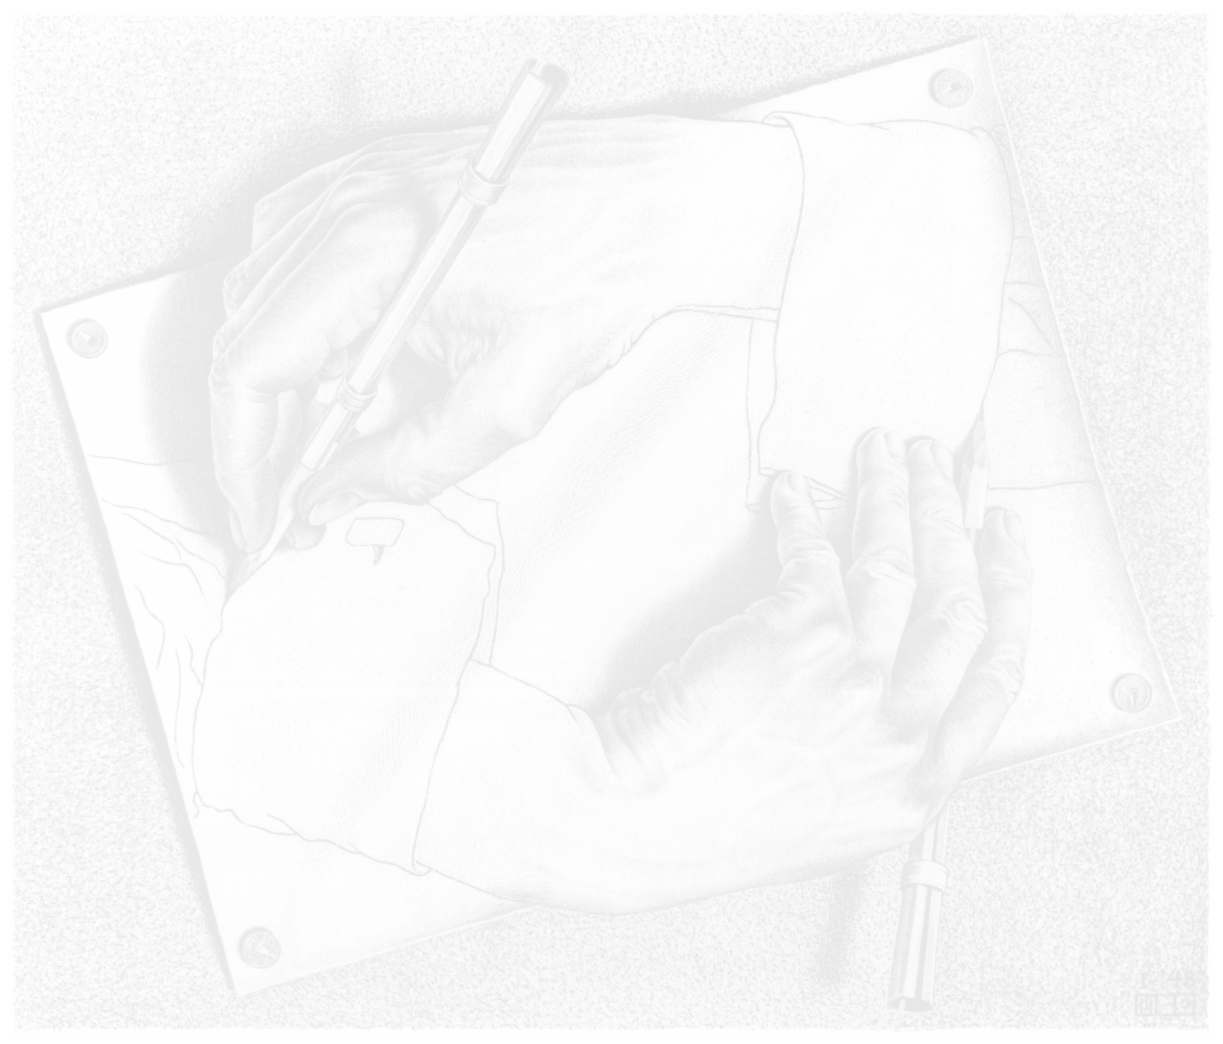
\includegraphics[width=\paperwidth, height=\paperheight]{./figure/escher_hands_tr.png}
%    }
}

%\usetheme{Hannover}
\usetheme{Copenhagen}
\usecolortheme{seahorse}
\usecolortheme{rose}
%\usetheme{Frankfurt}
%\usecolortheme{beetle}

%\useoutertheme[subsection=false]{smoothbars}
%\useoutertheme[subsection=false]{smoothtree}
\useoutertheme{shadow}
\setbeamercovered{dynamic}

\pgfdeclareimage[height=1cm]{logo}{figure/logo}
\logo{\pgfuseimage{logo}}

\begin{document}

%%%%%%%%%%%%%%%%%%%%%%%%%%%%%%%%%%%%%%%%%%%%%%%%%%%%%

\begin{frame}
\maketitle
\end{frame}

%%%%%%%%%%%%%%%%%%%%%%%%%%%%%%%%%%%%%%%%%%%%%%%%%%%%%

\begin{frame}
\frametitle{Outline}
	\tableofcontents
\end{frame}

%%%%%%%%%%%%%%%%%%%%%%%%%%%%%%%%%%%%%%%%%%%%%%%%%%%%%

\section{Introduzione}
\begin{frame}
\frametitle{Definizione}
In 1998 (the same year that HITS was born), Google founders Larry Page and Sergey Brin formulated
their PageRank concept and made it the basis for their search engine [15]. As stated on the Google web
site
By avoiding the inherent weaknesses of HITS, PageRank has been responsible for elevating Google to the
position of the world's preeminent search engine.
\end{frame}

%%%%%%%%%%%%%%%%%%%%%%%%%%%%%%%%%%%%%%%%%%%%%%%%%%%%%

\begin{frame}
	\frametitle{Definizione}
	\begin{itemize}
		\item Formulato nel 1998 da Larry Page e Sergey Brin
		\item Algoritmo di ricerca di Google : " The heart of our software is PageRank \texttrademark\dots it provides the basis for all of our web search tools.''
		\item Supera gli svantaggi di HITS
	\end{itemize}
\end{frame}

%%%%%%%%%%%%%%%%%%%%%%%%%%%%%%%%%%%%%%%%%%%%%%%%%%%%%

\begin{frame}
	\frametitle{Idea di base}
	I voti (link) da siti importanti dovrebbero avere un peso maggiore dei voti (link) da siti meno importanti, e l'importanza di un voto (link) da una qualunque sorgente dovrebbe essere attenuato dal numero dei siti che la sorgente vota
\end{frame}

%%%%%%%%%%%%%%%%%%%%%%%%%%%%%%%%%%%%%%%%%%%%%%%%%%%%%
\section{Funzionamento}
\begin{frame}
	\frametitle{Formalismo}
	\begin{itemize}
		\item Indicata con $P$ una generica pagina
		\item $B_P$ = \{ insieme delle pagine che puntano a P \}
		\item si definisce il punteggio $r(P)$ di $P$: $$\sum_{Q \in B_P}\frac{r(Q)}{|Q|}$$ dove \\ $B_P=\{$ insieme di tutte le pagine puntanti a $P\}$ \\ $|Q|$ = numero degli outlink di $Q$
	\end{itemize}
\end{frame}

%%%%%%%%%%%%%%%%%%%%%%%%%%%%%%%%%%%%%%%%%%%%%%%%%%%%%

\begin{frame}
	\begin{itemize}
		\item Se abbiamo \emph{n} pagine $P_1,P_2,\dots,P_n$ ed assegniamo a ciascuna pagina un arbitrario punteggio iniziale $r_0(P_i)=\frac{1}{n}$
		\item Il punteggio $r(P)$ può essere calcolato mediante la seguente iterazione: $$r_j(P_i)= \sum_{Q \in B_{P_i}}\frac{r_{j-1}(Q)}{|Q|} ~~~~~~~~ j=1,2,3,\dots$$
	\end{itemize}
\end{frame}


%%%%%%%%%%%%%%%%%%%%%%%%%%%%%%%%%%%%%%%%%%%%%%%%%%%%%

\begin{frame}
	\begin{itemize}
		\item Ponendo: $\pi_j^\intercal = (r_j(P_1),r_j(P_2),\dots,r_j(P_n))$\\
		\item \textbf{P} Matrice di Google per righe se:
		\begin{itemize}
			\item $p_{ij}= \frac{1}{P_i}$ se $P_i$ si connette con la pagina $P_j$
			\item $p_{ij}=0$ altrimenti
		\end{itemize}
		\item La precedente iterazione si può riscrivere come: $$ \pi_j^\intercal = \pi_{j-1}^\intercal P$$\\
		\item metodo delle potenze
	\end{itemize}
\end{frame}

%%%%%%%%%%%%%%%%%%%%%%%%%%%%%%%%%%%%%%%%%%%%%%%%%%%%%

\begin{frame}
	\frametitle{Esempio di graph web}
	\begin{columns}
		\begin{column}{0.4\textwidth}
				\begin{center}
					\begin{tikzpicture}[->,>=stealth',shorten >=1pt,auto,node distance=1.2cm,
					thick,main node/.style={circle,fill=yellow!80,draw,font=\sffamily\Large\bfseries}]
					
					\node[main node] (1) {1};
					\node (1a) [right of=1] {};
					\node[main node] (2) [right of=1a] {2};
					\node (3a) [below of=1] {};
					\node[main node] (3) [below of=1a] {3};
					\node (3b) [below of=2] {};
					\node[main node] (5) [below of=3b] {5};
					\node (5a) [below of=3] {};
					\node[main node] (4) [below of=3a] {4};
					\node[main node] (6) [below of=5a] {6};
					
					\path[every node/.style={font=\sffamily\small}]
					(2) edge [bend right] node [right] {} (1)
					(1) edge node [right] {} (2)
					(1) edge node [right] {} (3)
					(3) edge node [right] {} (4)
					(5) edge node [right] {} (3)
					(3) edge [bend right] node [right] {} (2)
					(2) edge node [right] {} (3)
					(5) edge node [right] {} (4)
					(4) edge [bend right] node [right] {} (5)
					(4) edge [bend right] node [right] {} (6)
					(6) edge [bend right] node [right] {} (5)
					;
					\end{tikzpicture}
				\end{center}
		\end{column}
		\begin{column}{0.6\textwidth}
			\vspace{1cm}
			Matrice Google per righe \textbf{P}
			$\textbf{P} = \begin{bmatrix}
			0           & \frac{1}{2} & \frac{1}{2}& 0          & 0          & 0           \\[0.3em]
			\frac{1}{2} & 0           & \frac{1}{2}& 0          & 0          & 0           \\[0.3em]
			0           & \frac{1}{2} & 0          & \frac{1}{2}& 0          & 0           \\[0.3em]
			0           & 0           & 0          & 0          & \frac{1}{2}& \frac{1}{2} \\[0.3em]
			0           & 0           & \frac{1}{2}& \frac{1}{2}& 0          & 0           \\[0.3em]
			0           & 0           & 0          & 0          & 0          & 1           \\[0.3em]
			\end{bmatrix}$
		\end{column}
	\end{columns}
\end{frame}

%%%%%%%%%%%%%%%%%%%%%%%%%%%%%%%%%%%%%%%%%%%%%%%%%%%%%

\begin{frame}
	\begin{itemize}
		\item Se il limite esiste, il vettore PageRank è definito $$ \pi^\intercal = \lim_{j\to\infty}\pi_j^\intercal$$
		\item la \emph{i}-sima componente del vettore PageRank è il punteggio(pagerank) della pagina $P_i$
		\item Per assicurare la convergenza del processo iterativo la matrice \emph{P} deve essere modificata
	\end{itemize}
\end{frame}

%%%%%%%%%%%%%%%%%%%%%%%%%%%%%%%%%%%%%%%%%%%%%%%%%%%%%

\begin{frame}
	\begin{itemize}
		\item La matrice di Google per righe \textbf{P} è 
		\begin{itemize}
			\item non-negativa
			\item somma degli elementi sulle righe pari a zero\footnote{nodi \emph{dangling}} o uno
		\end{itemize}
		\item Se la matrice \textbf{P} ha tutte le righe con somma pari a uno allora si parla di matrice stocastica:
		\begin{itemize}
			\item autovalore dominante uguale a 1
			\item iterazione PageRank converge all'autovettore sinistro normalizzato $\pi^\intercal=\pi^\intercal \textbf{P}$ t.c. $\pi^\intercal \mathbb{1} = 1$
		\end{itemize}
	\end{itemize}
\end{frame}

%%%%%%%%%%%%%%%%%%%%%%%%%%%%%%%%%%%%%%%%%%%%%%%%%%%%%

\begin{frame}
	\frametitle{Esempio nodo dangling}
	\begin{columns}
		\begin{column}{0.4\textwidth}
\begin{tikzpicture}[->,>=stealth',shorten >=1pt,auto,node distance=1.2cm,
thick,main node/.style={circle,fill=yellow!80,draw,font=\sffamily\Large\bfseries}]

\node[main node] (1) {1};
\node (1a) [right of=1] {};
\node[main node] (2) [right of=1a] {2};
\node (3a) [below of=1] {};
\node[main node] (3) [below of=1a] {3};
\node (3b) [below of=2] {};
\node[main node] (5) [below of=3b] {5};
\node (5a) [below of=3] {};
\node[main node] (4) [below of=3a] {4};
\node[main node,fill=red!60] (6) [below of=5a] {6};

\path[every node/.style={font=\sffamily\small}]
(2) edge [bend right] node [right] {} (1)
(1) edge node [right] {} (2)
(1) edge node [right] {} (3)
(3) edge node [right] {} (4)
(5) edge node [right] {} (3)
(3) edge [bend right] node [right] {} (2)
(2) edge node [right] {} (3)
(5) edge node [right] {} (4)
(4) edge [bend right] node [right] {} (5)
(4) edge [bend right] node [right] {} (6)
;
\end{tikzpicture}
		\end{column}
		\begin{column}{0.6\textwidth}
			\vspace{1cm}
			$\textbf{P} = \begin{bmatrix}
			0           & \frac{1}{2} & \frac{1}{2}& 0          & 0          & 0           \\[0.3em]
			\frac{1}{2} & 0           & \frac{1}{2}& 0          & 0          & 0           \\[0.3em]
			0           & \frac{1}{2} & 0          & \frac{1}{2}& 0          & 0           \\[0.3em]
			0           & 0           & 0          & 0          & \frac{1}{2}& \frac{1}{2} \\[0.3em]
			0           & 0           & \frac{1}{2}& \frac{1}{2}& 0          & 0           \\[0.3em]
			\textcolor{red}{0}&\textcolor{red}{0}&\textcolor{red}{0}&\textcolor{red}{0}&\textcolor{red}{0}& \textcolor{red}{0}\\[0.3em]
			\end{bmatrix}$
		\end{column}
	\end{columns}
	\textcolor{white}{s}
	\\
	Il nodo 6 è un nodo dangling in quando non ha outlink
\end{frame}

%%%%%%%%%%%%%%%%%%%%%%%%%%%%%%%%%%%%%%%%%%%%%%%%%%%%%
\begin{frame}
	\frametitle{Trasformazione Matrice di Google per righe}
	\begin{itemize}
		\item Stocastica
		\begin{itemize}
			\item Sostituire ad ogni riga nulla il vettore $\frac{\mathbb{1}^\intercal}{n}$
			\item La nuova matrice stocastica si indica con $\bar{\textbf{P}}$\\~\\
		\end{itemize}
		
		\item Irriducibile
				\begin{itemize}
					\item Aggiungere una matrice di perturbazione $\textbf{E} = \frac{\mathbb{11}^\intercal}{n}$
					\item La nuova matrice sarà uguale a  $$\bar{\bar{\textbf{P}}} = \alpha\bar{\textbf{P}} + (1-\alpha)\textbf{E} ~~~~~~~~ \alpha \in [0,1]$$
				\end{itemize}
	\end{itemize}
\end{frame}

%%%%%%%%%%%%%%%%%%%%%%%%%%%%%%%%%%%%%%%%%%%%%%%%%%%%%
\begin{frame}
	\begin{itemize}
		\item La matrice di Google attualmente utilizzata è ottenuta
		considerando la matrice di perturbazione  $\textbf{E} = \mathbb{1v}^\intercal$ dove $v^\intercal$ è un vettore di personalizzazione dell'utente $$\bar{\bar{\textbf{P}}} = \alpha\bar{\textbf{P}} + (1-\alpha)\mathbb{1v}^\intercal ~~~~~~~~ \alpha \in [0,1]$$
	\end{itemize}
\end{frame}

%%%%%%%%%%%%%%%%%%%%%%%%%%%%%%%%%%%%%%%%%%%%%%%%%%%%%
\section{Implementazione}
\begin{frame}
	\frametitle{Implementazione di PageRank}
	Data una query \emph{q}:
	\begin{enumerate}
		\item Determinare l'insieme di rilevanza della query creando il sottoinsieme di pagine contenenti i termini della query (\emph{indicizzazione inversa})
		\item Applicare il PageRank all'insieme di rilevanza di q per ottenere il rank delle pagine considerate (Ogni documento ha un punteggio PageRank indipendente dalla query)
	\end{enumerate}
\end{frame}
%%%%%%%%%%%%%%%%%%%%%%%%%%%%%%%%%%%%%%%%%%%%%%%%%%%%%
\begin{frame}
	\frametitle{Calcolo del vettore PageRank $\pi^\intercal$ relativo a $\bar{\bar{\textbf{P}}}$}
	\begin{enumerate}
		\item Specificare il parametro $\alpha$
		\item Porre $\pi_0^\intercal=\frac{\mathbb{1}^\intercal}{n}$
		\item Fissata la threshold, iterare fino alla convergenza l'equazione $$\pi_{k+1}^\intercal = \alpha \pi_{k+1}^\intercal \bar{\textbf{P}} + (1- \alpha) \mathbb{v}^\intercal  $$
	\end{enumerate}
\end{frame}
%%%%%%%%%%%%%%%%%%%%%%%%%%%%%%%%%%%%%%%%%%%%%%%%%%%%%
\section{Esempio}
\begin{frame}
	\frametitle{Esempio \dots}
	Consideriamo l'insieme di rilevanza composto da sei pagine web aventi la seguente struttura ad hyperlink
	\\~\\
	\begin{center}
	\begin{tikzpicture}[->,>=stealth',shorten >=1pt,auto,node distance=1.2cm,
	thick,main node/.style={circle,fill=yellow!80,draw,font=\sffamily\Large\bfseries}]
	
	\node[main node] (1) {1};
	\node (1a) [right of=1] {};
	\node[main node] (2) [right of=1a] {2};
	\node (3a) [below of=1] {};
	\node[main node] (3) [below of=1a] {3};
	\node (3b) [below of=2] {};
	\node[main node] (5) [below of=3b] {5};
	\node (5a) [below of=3] {};
	\node[main node] (6) [below of=3a] {6};
	\node[main node] (4) [below of=5a] {4};

	\path[every node/.style={font=\sffamily\small}]
	(1) edge node [right] {} (2)
	(1) edge [bend right] node [right] {} (3)
	(3) edge node [right] {} (1)
	(3) edge node [right] {} (2)
	(3) edge node [right] {} (5)
	(5) edge node [right] {} (6)
	(4) edge [bend right] node [right] {} (5)
	(5) edge node [right] {} (4)
	(4) edge node [right] {} (6)
	(6) edge [bend right] node [right] {} (4)
;
	\end{tikzpicture}
	\end{center}
\end{frame}
%%%%%%%%%%%%%%%%%%%%%%%%%%%%%%%%%%%%%%%%%%%%%%%%%%%%%
\begin{frame}
	\frametitle{\dots Esempio \dots}
	La matrice di Google per righe corrispondente al grafo sarà la seguente
	\\~\\
	\begin{center}
		$\textbf{P} = \begin{bmatrix}
		0           & \frac{1}{2} & \frac{1}{2}& 0          & 0          & 0           \\[0.3em]
		0           & 0           & 0          & 0          & 0          & 0           \\[0.3em]
		\frac{1}{3} & \frac{1}{3} & 0          & 0          & \frac{1}{3}& 0           \\[0.3em]
		0           & 0           & 0           & 0          & \frac{1}{2}& \frac{1}{2} \\[0.3em]
		0           & 0           & 0           & \frac{1}{2}& 0          & \frac{1}{2} \\[0.3em]
		0           & 0           & 0           & 1          & 0          & 0           \\[0.3em]
		\end{bmatrix}$
	\end{center}
\end{frame}

%%%%%%%%%%%%%%%%%%%%%%%%%%%%%%%%%%%%%%%%%%%%%%%%%%%%%
\begin{frame}
	\frametitle{\dots Esempio \dots}
	Considerato che il nodo 2 è un nodo dangling allora sarà necessario trasformarla in matrice stocastica
	\\~
	\begin{center}
	$\bar{\textbf{P}} = \begin{bmatrix}
	0           & \frac{1}{2} & \frac{1}{2} & 0          & 0          & 0           \\[0.3em]
	\textcolor{red}{\frac{1}{6}} & \textcolor{red}{\frac{1}{6}} & \textcolor{red}{\frac{1}{6}} & \textcolor{red}{\frac{1}{6}}& \textcolor{red}{\frac{1}{6}}& \textcolor{red}{\frac{1}{6}} \\[0.3em]
	\frac{1}{3} & \frac{1}{3} & 0           & 0          & \frac{1}{3}& 0           \\[0.3em]
	0           & 0           & 0           & 0          & \frac{1}{2}& \frac{1}{2} \\[0.3em]
	0           & 0           & 0           & \frac{1}{2}& 0          & \frac{1}{2} \\[0.3em]
	0           & 0           & 0           & 1          & 0          & 0           \\[0.3em]
	\end{bmatrix}$
	\end{center}
\end{frame}
%%%%%%%%%%%%%%%%%%%%%%%%%%%%%%%%%%%%%%%%%%%%%%%%%%%%%
\begin{frame}
	\frametitle{\dots Esempio\dots}
	La matrice stocastica ottenuta è una matrice riducibile
	\\~\\
	\begin{center}
	$\bar{\textbf{P}} = \begin{bmatrix}
	0           & \frac{1}{2} & \frac{1}{2} & 0          & 0          & 0           \\[0.3em]
	\frac{1}{6} & \frac{1}{6} & \frac{1}{6} & \frac{1}{6}& \frac{1}{6}& \frac{1}{6} \\[0.3em]
	\frac{1}{3} & \frac{1}{3} & 0           & 0          & \frac{1}{3}& 0           \\[0.3em]
	\textcolor{red}{0}& \textcolor{red}{0} &\textcolor{red}{0}& 0          & \frac{1}{2}& \frac{1}{2} \\[0.3em]
	\textcolor{red}{0}& \textcolor{red}{0} &\textcolor{red}{0}& \frac{1}{2}& 0          & \frac{1}{2} \\[0.3em]
	\textcolor{red}{0}& \textcolor{red}{0} &\textcolor{red}{0}& 1          & 0          & 0           \\[0.3em]
	\end{bmatrix}$
	\end{center}
\end{frame}
%%%%%%%%%%%%%%%%%%%%%%%%%%%%%%%%%%%%%%%%%%%%%%%%%%%%%
\begin{frame}
	\frametitle{\dots Esempio \dots}
	Per ottenere una matrice irriducibile scegliamo arbitrariamente il parametro $\alpha=0.9$ da applicare alla formula \footnote{$\bar{\bar{\textbf{P}}} = \alpha\bar{\textbf{P}} + \frac{(1-\alpha)\mathbb{11}^\intercal}{n}$}
	$$\bar{\bar{\textbf{P}}} = 0.9*\bar{\textbf{P}} + \frac{0.1*\mathbb{11}^\intercal}{6}$$
	\begin{center}
		$\bar{\bar{\textbf{P}}} = \begin{bmatrix}
		\frac{1}{60} & \frac{7}{15}  & \frac{7}{15} & \frac{1}{60} &\frac{1}{60} &\frac{1}{60} \\[0.3em]
		\frac{1}{6}  & \frac{1}{6}   & \frac{1}{6}  & \frac{1}{6}  &\frac{1}{6}  &\frac{1}{6}  \\[0.3em]
		\frac{19}{60}& \frac{19}{60} & \frac{1}{60} & \frac{1}{60} &\frac{19}{60}&\frac{1}{60} \\[0.3em]
		\frac{1}{60} & \frac{1}{60}  & \frac{1}{60} & \frac{1}{60} &\frac{7}{15} &\frac{7}{15} \\[0.3em]
		\frac{1}{60} & \frac{1}{60}  & \frac{1}{60} & \frac{7}{15} &\frac{1}{60} &\frac{7}{15} \\[0.3em]
		\frac{1}{60} & \frac{1}{60}  & \frac{1}{60} & \frac{11}{12}&\frac{1}{60} &\frac{1}{60} \\[0.3em]
		\end{bmatrix}$
	\end{center}
\end{frame}
%%%%%%%%%%%%%%%%%%%%%%%%%%%%%%%%%%%%%%%%%%%%%%%%%%%%%
\begin{frame}
	\frametitle{\dots Esempio}
	\begin{itemize}
		\item Il vettore di PageRank associato alla precedente matrice sarà $$\pi^\intercal=(0.3721~~0.05396~~0.0415~~0.375~~0.206~~0.286)$$
		\item Vettore indipendente dalla query
	\end{itemize}
\end{frame}
%%%%%%%%%%%%%%%%%%%%%%%%%%%%%%%%%%%%%%%%%%%%%%%%%%%%%
\begin{frame}
	\frametitle{Esempio di raccomandazione}
	\begin{itemize}
		\item Data una query contenente i termini \emph{t1} e \emph{t2}
		\item Calcoliamo l'insieme di rilevanza per la query $q=(t1,t2)$
		\begin{itemize}
			\item Insieme di rilevanza \{1~3~4~6\}
		\end{itemize}
		\item I PageRank dei 4 documenti possono essere confrontati per individuare quale dei documenti è il più rilevante
		\begin{itemize}
			\item ordinare le componenti del vettore pagerank associate ai documenti selezionati in modo decrescente
			\item $\pi_4~\pi_6~\pi_3~\pi_1$
			\item doc4 $\longrightarrow$ documento più rilevante
			\item seguono doc6, doc3, doc1
		\end{itemize}
	\end{itemize}
\end{frame}
%%%%%%%%%%%%%%%%%%%%%%%%%%%%%%%%%%%%%%%%%%%%%%%%%%%%%
\section{}
\begin{frame}
%	basicstyle=\fontsize{8}{10}\selectfont \ttfamily,%
\begin{center}
Grazie per l'attenzione.
\end{center}
\end{frame}
\end{document}
